% !TEX root =  ../supplementary.tex
\section{Risk Predictions for Reclassification}
\label{sec:param_estimates_jm_fit_prias}
Let us assume a new patient $j$, for whom we need to estimate the risk of reclassification. Let his current follow-up visit time be $s$, latest time of biopsy be $t$, observed vector PSA measurements be $\mathcal{Y}_{j}(s)$. The combined information from the observed data about the time of reclassification, is given by the following posterior predictive distribution $g(T^*_j)$ of his time $T^*_j$ of reclassification:
\begin{equation*}
\label{eq:post_pred_dist}
\begin{aligned}
g(T^*_j) &= p\big\{T^*_j \mid T^*_j > t, \mathcal{Y}_{j}(s), \mathcal{D}_n\big\}\\
&= \int \int p\big(T^*_j \mid T^*_j > t, \boldsymbol{b}_j, \boldsymbol{\theta}\big)\\
&\times p\big\{\boldsymbol{b}_j \mid T^*_j>t, \mathcal{Y}_{j}(s), \boldsymbol{\theta}\big\}p\big(\boldsymbol{\theta} \mid \mathcal{D}_n\big) \mathrm{d} \boldsymbol{b}_j \mathrm{d} \boldsymbol{\theta}.
\end{aligned}
\end{equation*}
The distribution $g(T^*_j)$ depends not only depends on the observed data of the patient $T^*_j > t, \mathcal{Y}_{j}(s)$, but also depends on the information from the PRIAS dataset $\mathcal{D}_n$. To this the the posterior distribution of random effects $\boldsymbol{b}_j$ and posterior distribution of the vector of all parameters $\boldsymbol{\theta}$ are utilized, respectively. The distribution $g(T^*_j)$ can be estimated as detailed in \citet{rizopoulos2017dynamic}. Since, majority of the prostate cancer patients may not obtain reclassification in the current follow-up period of PRIAS (thirteen years), $g(T^*_j)$ can only be estimated for time points falling within the thirteen year follow-up. 

The cumulative risk of reclassification can be derived from $g(T^*_j)$ as given in \citep{rizopoulos2017dynamic}. It is given by:
\begin{equation}
\label{eq:dynamic_risk_prob}
R_j(u \mid t,s) = \mbox{Pr}\big\{T^*_j > u \mid T^*_j > t, \mathcal{Y}_{j}(s), \mathcal{D}_n\big\}, \quad u \geq t.
\end{equation}
The personalized risk profile of the patient (see Panel~C, Figure~\ref{fig:dynrisk_plot_102}) updates as more data is gathered over follow-up visits. 

\begin{figure}
\centerline{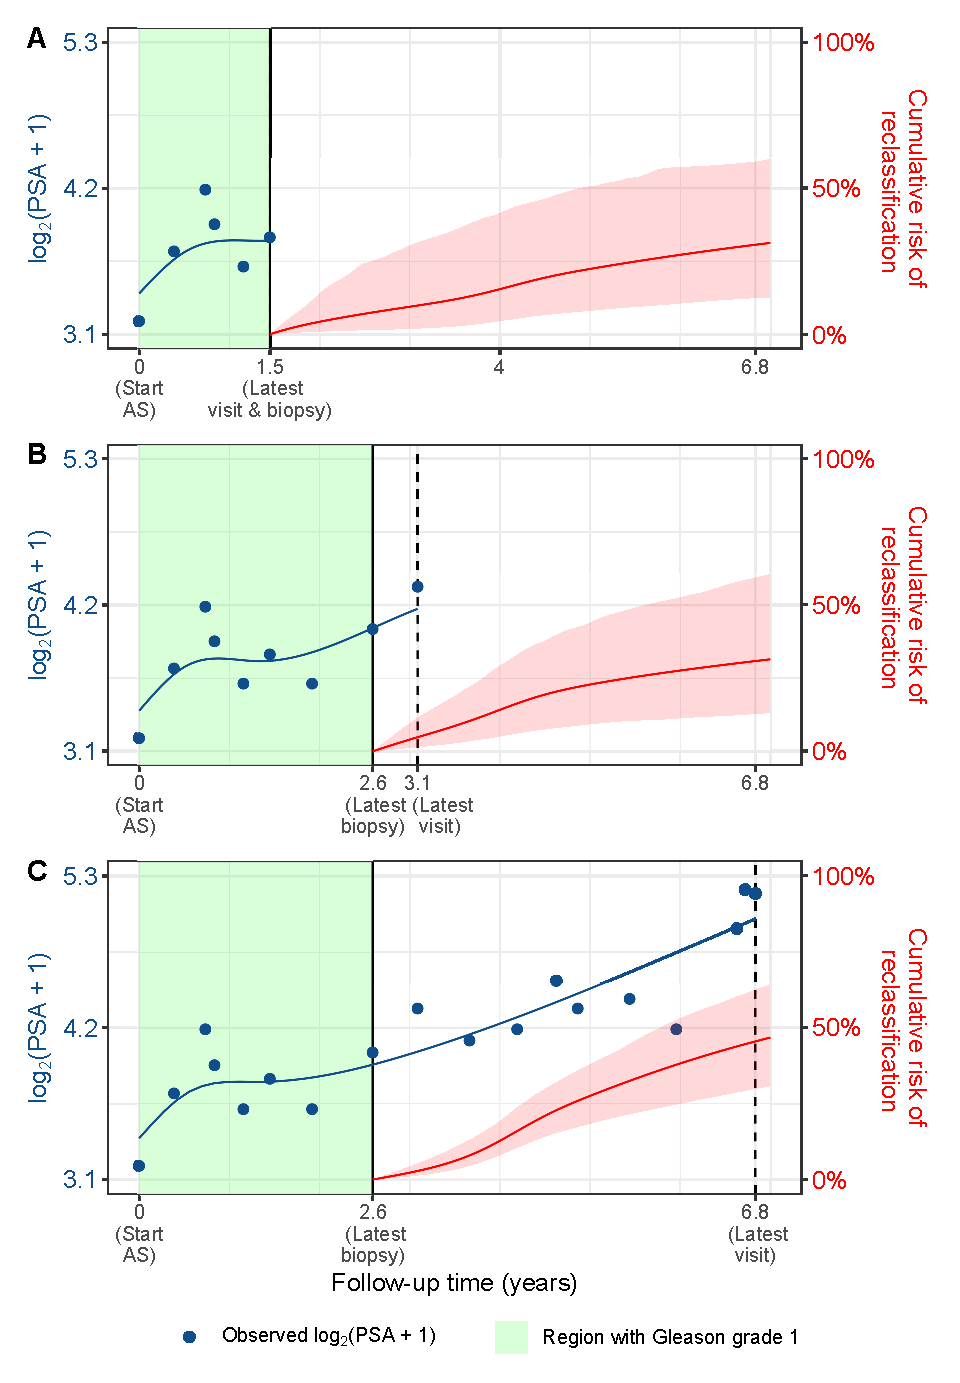
\includegraphics[width=\columnwidth]{images/dynrisk_plot_102.eps}}
\caption{\textbf{Cumulative risk of (reclassification) changing dynamically over follow-up} as more patient data is gathered. The three \textbf{Panels~A,B~and~C:} are ordered by the time of the latest visit (dashed vertical black line) of a new patient. At each of the latest follow-up visits, we combine the accumulated PSA measurements (shown in blue), and latest time of negative biopsy (solid vertical black line) to obtain the updated cumulative risk profile (shown in red) of the patient.}
\label{fig:dynrisk_plot_102}
\end{figure}

\clearpage
\subsection{Validation of Risk Predictions}
We wanted to check the discrimination and calibration of our model. At the same time we also wanted to check if our model could be used in other cohorts. To this end, we validated the predictions of reclassification internally within the PRIAS dataset, as well as externally in largest five AS cohorts from the GAP3 database \citep{gap3_2018}. These are the University of Toronto AS (Toronto), Johns Hopkins AS (Hopkins), Memorial Sloan Kettering Cancer Center AS (MSKCC), King's College London AS (KCL), and Michigan Urological Surgery Improvement Collaborative AS (MUSIC). In all of these cohorts, we calculated the area under the receiver operating characteristic curve or AUC \cite{rizopoulos2017dynamic} as a measure of discrimination between patients who obtain reclassification and those do not obtain reclassification. We also calculated root mean squared prediction error or RMSPE \cite{rizopoulos2017dynamic} as a measure of calibration. Both AUC and RMSPE take a value between 0 and 1. Ideally RMSPE should be 0 and AUC should 1. In addition, it is preferred that AUC $>$ 0.5 because an AUC $\leq$ 0.5 indicates that the model performs worse than random discrimination. Since AS studies are longitudinal in nature, AUC and RMSPE are also time dependent. More specifically, given the time of latest biopsy $t$, and history of PSA measurements up to time $s$, we calculate AUC and RMSPE for a medically relevant time frame $(t, s]$, within which the occurrence of reclassification is of interest. In the case of prostate cancer, at any point in time $s$ it is of interest to identify patients who may have obtained reclassification in the last one year $(s-1, s]$. That is we set $t=s-1$. We then calculate AUC and RMSPE at a gap of every six months (follow-up schedule of PRIAS) until year five (95-percentile of the observed times of reclassification), that is, $s \epsilon \{1, 1.5, \ldots, 5\}$ years. The resulting estimates are summarized in Figure~\ref{fig:auc_pe}, and in Table~\ref{tab:AUC_PE_PRIAS} to Table~\ref{tab:AUC_PE_MUSIC}.

\begin{figure}
\centerline{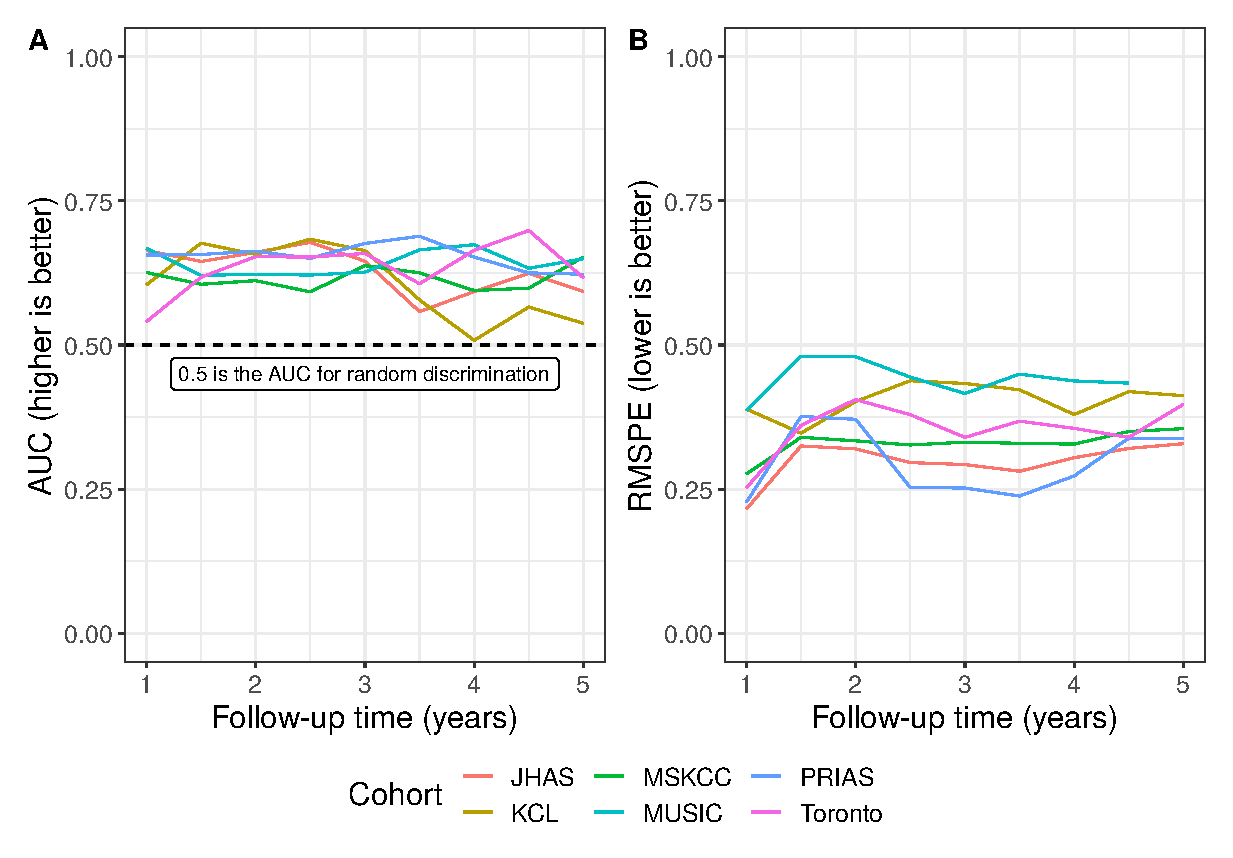
\includegraphics[width=\columnwidth]{images/auc_pe.eps}}
\caption{\textbf{Validation of predictions of Gleason $\geq$ 7 (reclassification)}. In \textbf{Panel~A} we can see that the time dependent area under the receiver operating characteristic curve or AUC (measure of discrimination) is above 0.5 in PRIAS (internal validation), and in Toronto, JHAS, MSKCC, KCL, and MUSIC AS cohorts (external validation). In \textbf{Panel~B} we can see that the time dependent root mean squared prediction error or RMSPE (measure of calibration) is similar for PRIAS, and JHAS and Toronto cohorts. The bootstrapped 95\% confidence interval for these estimates are presented in Table~\ref{tab:AUC_PE_PRIAS} to Table~\ref{tab:AUC_PE_KCL}. Full names of Cohorts are \textit{PRIAS}: Prostate Cancer International Active Surveillance, \textit{Toronto}: University of Toronto Active Surveillance, \textit{JHAS}: Johns Hopkins Active Surveillance, \textit{MSKCC}: Memorial Sloan Kettering Cancer Center Active Surveillance, \textit{KCL}: King's College London Active Surveillance, \textit{MUSIC}: Michigan Urological Surgery Improvement Collaborative Active Surveillance.}
\label{fig:auc_pe}
\end{figure}

\begin{table}[!htb]
\small\sf\centering
\caption{\textbf{Internal Validation of predictions of Gleason $\geq$ 7 (reclassification) in PRIAS cohort}. The area under the receiver operating characteristic curve or AUC (measure of discrimination) root mean squared prediction error or RMSPE (measure of calibration) are calculated over the follow-up period at a gap of 6 months. In addition bootstrapped 95\% confidence intervals (CI) are also presented.}
\label{tab:AUC_PE_PRIAS}
\begin{tabular}{r|r|r}
\hline
\hline
Follow-up period (years) & AUC (95\% CI) & RMSPE (95\%CI)\\ 
\hline
0.0 to 1.0 & 0.656 [0.623, 0.690] & 0.227 [0.223, 0.236]\\
0.5 to 1.5 & 0.657 [0.641, 0.671] & 0.376 [0.371, 0.382]\\
1.0 to 2.0 & 0.663 [0.651, 0.678] & 0.371 [0.364, 0.379]\\
1.5 to 2.5 & 0.650 [0.600, 0.684] & 0.253 [0.245, 0.263]\\
2.0 to 3.0 & 0.676 [0.641, 0.725] & 0.252 [0.241, 0.262]\\
2.5 to 3.5 & 0.689 [0.629, 0.732] & 0.238 [0.224, 0.251]\\
3.0 to 4.0 & 0.652 [0.614, 0.709] & 0.273 [0.263, 0.285]\\
3.5 to 4.5 & 0.625 [0.591, 0.663] & 0.338 [0.326, 0.349]\\
4.0 to 5.0 & 0.623 [0.587, 0.657] & 0.338 [0.325, 0.350]\\
\hline
\end{tabular}	
\end{table}

\begin{table}[!htb]
\small\sf\centering
\caption{\textbf{External Validation of predictions of Gleason $\geq$ 7 (reclassification) in University of Toronto Active Surveillance cohort}. The area under the receiver operating characteristic curve or AUC (measure of discrimination) root mean squared prediction error or RMSPE (measure of calibration) are calculated over the follow-up period at a gap of 6 months. In addition bootstrapped 95\% confidence intervals (CI) are also presented.}
\label{tab:AUC_PE_Toronto}
\begin{tabular}{r|r|r}
\hline
\hline
Follow-up period (years) & AUC (95\% CI) & RMSPE (95\%CI)\\ 
\hline
0.0 to 1.0 & 0.540 [0.493, 0.595] & 0.252 [0.236, 0.272]\\
0.5 to 1.5 & 0.618 [0.562, 0.660] & 0.361 [0.350, 0.373]\\
1.0 to 2.0 & 0.653 [0.580, 0.719] & 0.405 [0.384, 0.428]\\
1.5 to 2.5 & 0.652 [0.596, 0.727] & 0.379 [0.358, 0.408]\\
2.0 to 3.0 & 0.659 [0.565, 0.743] & 0.340 [0.303, 0.369]\\
2.5 to 3.5 & 0.606 [0.548, 0.676] & 0.368 [0.340, 0.401]\\
3.0 to 4.0 & 0.664 [0.583, 0.736] & 0.355 [0.324, 0.391]\\
3.5 to 4.5 & 0.699 [0.610, 0.773] & 0.340 [0.310, 0.374]\\
4.0 to 5.0 & 0.617 [0.546, 0.705] & 0.397 [0.355, 0.425]\\
\hline
\end{tabular}	
\end{table}

\begin{table}[!htb]
\small\sf\centering
\caption{\textbf{External Validation of predictions of Gleason $\geq$ 7 (reclassification) in Johns Hopkins Active Surveillance cohort}. The area under the receiver operating characteristic curve or AUC (measure of discrimination) root mean squared prediction error or RMSPE (measure of calibration) are calculated over the follow-up period at a gap of 6 months. In addition bootstrapped 95\% confidence intervals (CI) are also presented.}
\label{tab:AUC_PE_JHAS}
\begin{tabular}{r|r|r}
\hline
\hline
Follow-up period (years) & AUC (95\% CI) & RMSPE (95\%CI)\\ 
\hline
0.0 to 1.0 & 0.664 [0.604, 0.743] & 0.216 [0.198, 0.236]\\
0.5 to 1.5 & 0.645 [0.597, 0.695] & 0.325 [0.310, 0.339]\\
1.0 to 2.0 & 0.661 [0.615, 0.707] & 0.320 [0.300, 0.335]\\
1.5 to 2.5 & 0.678 [0.587, 0.736] & 0.296 [0.277, 0.312]\\
2.0 to 3.0 & 0.645 [0.595, 0.701] & 0.293 [0.268, 0.317]\\
2.5 to 3.5 & 0.558 [0.445, 0.622] & 0.281 [0.256, 0.307]\\
3.0 to 4.0 & 0.593 [0.498, 0.693] & 0.305 [0.281, 0.329]\\
3.5 to 4.5 & 0.624 [0.527, 0.690] & 0.321 [0.294, 0.340]\\
4.0 to 5.0 & 0.593 [0.483, 0.694] & 0.329 [0.306, 0.352]\\
\hline
\end{tabular}	
\end{table}

\begin{table}[!htb]
\small\sf\centering
\caption{\textbf{External Validation of predictions of Gleason $\geq$ 7 (reclassification) in Memorial Sloan Kettering Cancer Center Active Surveillance cohort}. The area under the receiver operating characteristic curve or AUC (measure of discrimination) root mean squared prediction error or RMSPE (measure of calibration) are calculated over the follow-up period at a gap of 6 months. In addition bootstrapped 95\% confidence intervals (CI) are also presented.}
\label{tab:AUC_PE_MSKCC}
\begin{tabular}{r|r|r}
\hline
\hline
Follow-up period (years) & AUC (95\% CI) & RMSPE (95\%CI)\\ 
\hline
0.0 to 1.0 & 0.626 [0.558, 0.681]  & 0.276 [0.260, 0.297]\\
0.5 to 1.5 & 0.605 [0.539, 0.666]  & 0.340 [0.321, 0.360]\\
1.0 to 2.0 & 0.612 [0.564, 0.672]  & 0.334 [0.316, 0.350]\\
1.5 to 2.5 & 0.592 [0.502, 0.670]  & 0.327 [0.306, 0.345]\\
2.0 to 3.0 & 0.638 [0.548, 0.720]  & 0.332 [0.304, 0.363]\\
2.5 to 3.5 & 0.625 [0.542, 0.717]  & 0.330 [0.303, 0.371]\\
3.0 to 4.0 & 0.594 [0.511, 0.655]  & 0.328 [0.281, 0.368]\\
3.5 to 4.5 & 0.599 [0.481, 0.740]  & 0.350 [0.312, 0.373]\\
4.0 to 5.0 & 0.653 [0.562, 0.724]  & 0.355 [0.320, 0.380]\\
\hline
\end{tabular}	
\end{table}

\begin{table}[!htb]
\small\sf\centering
\caption{\textbf{External Validation of predictions of Gleason $\geq$ 7 (reclassification) in King's College London Active Surveillance cohort}. The area under the receiver operating characteristic curve or AUC (measure of discrimination) root mean squared prediction error or RMSPE (measure of calibration) are calculated over the follow-up period at a gap of 6 months. In addition bootstrapped 95\% confidence intervals (CI) are also presented.}
\label{tab:AUC_PE_KCL}
\begin{tabular}{r|r|r}
\hline
\hline
Follow-up period (years) & AUC (95\% CI) & RMSPE (95\%CI)\\ 
\hline
0.0 to 1.0 & 0.604 [0.548, 0.663] & 0.389 [0.366, 0.411]\\
0.5 to 1.5 & 0.676 [0.603, 0.744] & 0.347 [0.328, 0.372]\\
1.0 to 2.0 & 0.657 [0.578, 0.728] & 0.402 [0.368, 0.426]\\
1.5 to 2.5 & 0.683 [0.595, 0.773] & 0.438 [0.395, 0.469]\\
2.0 to 3.0 & 0.664 [0.576, 0.735] & 0.433 [0.396, 0.467]\\
2.5 to 3.5 & 0.578 [0.443, 0.712] & 0.422 [0.345, 0.479]\\
3.0 to 4.0 & 0.508 [0.358, 0.670] & 0.380 [0.313, 0.452]\\
3.5 to 4.5 & 0.566 [0.346, 0.776] & 0.419 [0.354, 0.484]\\
4.0 to 5.0 & 0.538 [0.295, 0.759] & 0.412 [0.345, 0.470]\\
\hline
\end{tabular}	
\end{table}

\begin{table}[!htb]
\small\sf\centering
\caption{\textbf{External Validation of predictions of Gleason $\geq$ 7 (reclassification) in Michigan Urological Surgery Improvement Collaborative Active Surveillance cohort}. The area under the receiver operating characteristic curve or AUC (measure of discrimination) root mean squared prediction error or RMSPE (measure of calibration) are calculated over the follow-up period at a gap of 6 months. In addition bootstrapped 95\% confidence intervals (CI) are also presented.}
\label{tab:AUC_PE_MUSIC}
\begin{tabular}{r|r|r}
\hline
\hline
Follow-up period (years) & AUC (95\% CI) & RMSPE (95\%CI)\\ 
\hline
0.0 to 1.0 & 0.667 [0.616, 0.703] & 0.387 [0.369, 0.409]\\
0.5 to 1.5 & 0.620 [0.566, 0.646] & 0.481 [0.462, 0.495]\\
1.0 to 2.0 & 0.623 [0.569, 0.666] & 0.480 [0.459, 0.501]\\
1.5 to 2.5 & 0.621 [0.580, 0.677] & 0.444 [0.418, 0.472]\\
2.0 to 3.0 & 0.626 [0.464, 0.710] & 0.416 [0.376, 0.459]\\
2.5 to 3.5 & 0.665 [0.554, 0.796] & 0.449 [0.390, 0.493]\\
3.0 to 4.0 & 0.674 [0.540, 0.757] & 0.438 [0.374, 0.483]\\
3.5 to 4.5 & 0.633 [0.410, 0.865] & 0.434 [0.346, 0.485]\\
4.0 to 5.0 & 0.650 [0.248, 0.946] & --    [--   , --   ]\\
\hline
\end{tabular}	
\end{table}